\chapter{Assembling programming environment}

% SPI wire programming

\subsection{Bug and limitations}

% connected to TOS build

\section{Mspdebug}

\section{Printf library}
\label{sec:printf_library}

When a code is first written, more often than not, it doesn't work as
expected. Unit testing helps, but often errors arise from making false
assumptions, and these may be reflected in tests as well. In such
case, only observing real behaviour will lead to fixing the issue.

But how to observe the behaviour of a node after it has been flashed
with new executable image?

One obvious source of information would be blinking LEDs on the board.
In case of the chronos watch, which has no LEDs, we may use the LCD
display, to even better results. But only small amount of information
can be retrieved through this channel. The next idea is to use
mspdebug tool mentioned before.  However if you ask a computer
programmer which tool he most commonly uses to find out what's
happening in his program, \emph{the debugger} will be his second
answer. The first would be \emph{printf}.

TinyOS has a convenient printf library that allows sending text
messages from running device to the PC, and display them on a console.
It's use is simple and comprises of following steps:

\begin{itemize}
  \item Include the printf library files to the build by adding
    following line to your Makefile:

    \texttt{CFLAGS += -I\$(TOSDIR)/lib/printf}

  \item Instantiate printf components in your application
    configuration. This step depends on which implementation of
    printf you choose. See below for details.

  \item Add following include in the file you wish to use printf in:

    \texttt{\#include ``printf.h''}

  \item Use \texttt{printf} statement to display messages and
    occasionally \texttt{printfflush} to ensure that they are not stuck
    in a buffer.

    \texttt{printf(``Value is \%d\textbackslash n'', value);} \\
    \texttt{printfflush();}

  \item To receive the messages you will need to run the printf
    client. This also depends on which implementation of print you
    choose.
\end{itemize}

Before we delve in to the specific implementations there's a warning
regarding printf buffering. Only after the buffer is filled or when
you call \texttt{printfflush} does the data get actually sent to the
PC. This isn't however immediate. If you very quickly print more text
than the capacity of the buffer, some of the messages will be lost!
Also note that \texttt{printfflush} is non-blocking and after calling
it, the buffer may still be overfilled for a while, and thus messages
may still get lost.

To overcome this,  you can shorten your messages or slow down printing
rate to ensure enough time to transmit current contents of the buffer.
Also you can increase the size of the buffer, which is set to 250 by
default, in \emph{print.h} header.

\subsection{Mspdebug printf}

\subsection{Radio printf}

\subsection{Serial port printf}
Third version of the printf library uses the serial port connection to
communicate with the PC. On the watch end it uses the UART (Universal
Asynchronous Receiver/Transmitter) hardware driver. This has both
serious advantages and a disadvantage.

Main advantage is, that serial communication is most reliable and best
supported way of sending printf messages in TinyOS. For example the
PrintfClient tool that comes with vanilla TinyOS, handles receiving
the packets and displaying them in the console. Also it is the least
intrusive one, since it neither requires halting the MCU nor sending
packets through the radio transceiver.

Main drawback however is that Texas Instruments did not make the UART
pins easily accessible on the chronos circuit board and certain
hardware modification is necessary.  It is described in appendix
\ref{appendix:uard_pins}. We will further assume that is has been
applied to the watch.

To enable this version of printf library you need to augment
instructions given in section \ref{sec:printf_library} with following
steps:

\begin{itemize}
  \item Instantiate these components in your application configuration:

  \texttt{components PrintfC, SerialStartC;}

  \item Connect the watch with hardware modification described in
    appendix \ref{appendix:uart_pins} to the USB debug dongle and
    connect the dongle to the PC.

  \item To receive messages run PrintfClient:

  \texttt{java net.tinyos.tools.PrintfClient -comm serial@/dev/ttyACM0:chronos}

  Note that watch may have shown in \texttt{\textbackslash dev} under
  different name, most commonly
  \texttt{\textbackslash dev\textbackslash ttyACM1}
\end{itemize}

\section{Eclipse integrated development environment}

The most practical way to work with TinyOS code is using the Eclipse
IDE. Some great work was done on that field, resulting in the Yeti 2
plugin. It supports TinyOS application and platform development,
providing many features. Below we'll describe the most important ones.

Firstly, in editor, there is some very good {\bf code completion} available
which eases writing both module and configuration files. It completes
component instantiations and connections. Also it completes interface
calls, function calls and variable names, and after adding a
\texttt{uses} or \texttt{provides} declaration, it offers to create
command stubs. These features are best shown on the following series of
figures - \ref{fig:first_compl} through \ref{fig:last_compl}.

\begin{figure}[h]
  \centering
  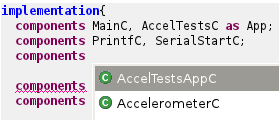
\includegraphics[width=0.85\textwidth]{img/eclipse_compl1.png}
  \caption{Component instantiation completion.}
  \label{fig:first_compl}
\end{figure}

\begin{figure}[h]
  \centering
  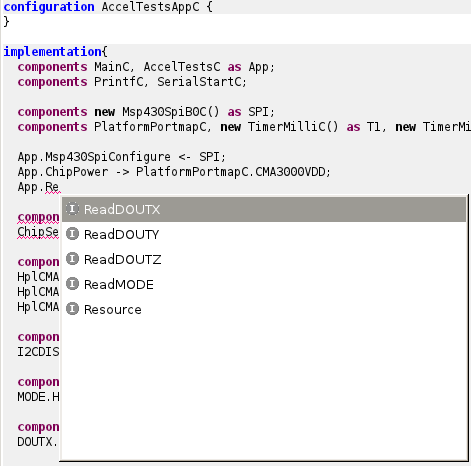
\includegraphics[width=0.8\textwidth]{img/eclipse_compl2.png}
  \caption{User connection completion.}
\end{figure}

\begin{figure}[h]
  \centering
  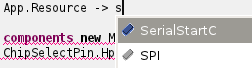
\includegraphics[width=0.9\textwidth]{img/eclipse_compl3.png}
  \caption{Provider connection completion.}
\end{figure}

\begin{figure}[h]
  \centering
  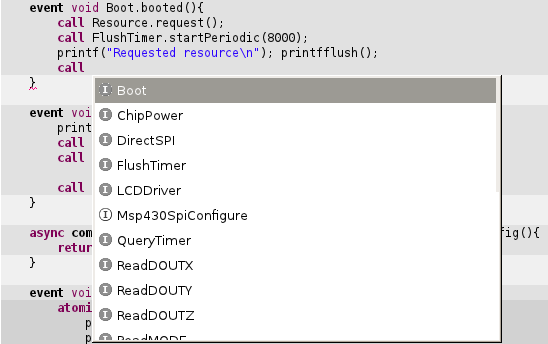
\includegraphics[width=0.9\textwidth]{img/eclipse_compl4.png}
  \caption{Interface completion.}
\end{figure}

\begin{figure}[h]
  \centering
  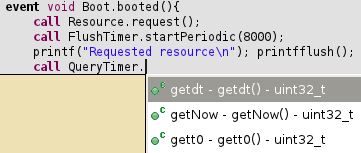
\includegraphics[width=0.9\textwidth]{img/eclipse_compl5.png}
  \caption{Command completion.}
\end{figure}

\begin{figure}[h]
  \centering
  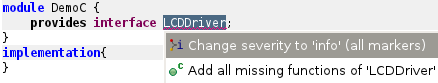
\includegraphics[width=0.9\textwidth]{img/eclipse_compl6.png}
  \caption{Command stubs generation.}
  \label{fig:last_compl}
\end{figure}

Another very useful feature, especially for a new developer wishing to
familiarize himself with TinyOS structure is the {\bf component
explorer}. It graphically displays components instantiated and
interconnected in configurations. Interfaces can be viewed as well.
Starting at the top level application configuration, every part of
it's code can be reached. This is by far the most efficient way to
explore the call hierarchy and find where particular functions are
implemented. Example of the PrintfC configuration, viewed through
the component explorer is shown in figure
\ref{fig:eclipse_compexp}.

\begin{figure}[h]
  \centering
  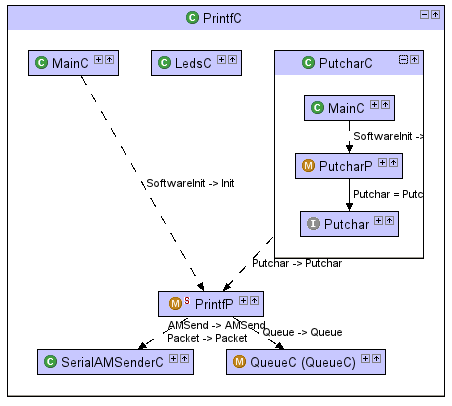
\includegraphics[width=0.7\textwidth]{img/eclipse_compexp.png}
  \caption{Component explorer showing PrintfC configuration.}
  \label{fig:eclipse_compexp}
\end{figure}

The eclipse editor also gives many warnings about the code without
triggering compilation. Moreover many of these useful warnings are not
raised by NesC compiler, which is an added value. 

Last but not least useful part of Yeti 2 is {\bf the debugger}. The
chains of tools needed to debug applications on the chronos watch is
long, but running them is as easy as pressing a button in the IDE. At
the lowest level, the \emph{mspdebug} communicates with the watch
through the USB debugging dongle. It runs a GDB Server to which newer
versions of \emph{msp430-gdb} are able to connect. Eclipse runs this
last executable and forms practical data views, reading crude data
from GDB. Here is a list of most useful views and features:
\begin{itemize}
  \item Single stepping through code in NesC editor.
  \item Call stack view.
  \item Breakpoints list (though limited to 3 active at any moment).
  \item Disassembly view.
  \item Raw memory view.
  \item Registers view.
  \item Local variables view.
  \item Module variables view.
\end{itemize}

There are many other features not mentioned here, most of which are
standard to Eclipse IDE and expected to be available for any supported
programming language.

\section{Other tools}

% vim syntax color and indent

% virtual machine

% Vim settings:
% vim: set textwidth=70:
% vim: set fo+=t:
